\documentclass[14pt,compress]{beamer}
\usepackage[spanish]{babel}
\usepackage[utf8]{inputenc}
\usepackage{presento}
\usepackage{comment}

\makeatletter
\newcommand{\vast}{\bBigg@{4}}
\newcommand{\Vast}{\bBigg@{5}}
\makeatother

%configuration file
%\setbeamercolor{title}{fg=DarkRed}
%\setbeamercolor{frametitle}{fg=DarkRed}
\setbeamercolor{normal text}{fg=darkgray}
\usebeamercolor[fg]{normal text}
%\setbeamercolor{block title}{fg=black,bg=Fern!25!white}
%\setbeamercolor{block body}{fg=black,bg=Fern!25!white}
%\setbeamercolor{alerted text}{fg=AlertColor}
%\setbeamercolor{itemize item}{fg=Charcoal}

\usepackage[font={color=dimgray},figurename={ },labelfont={ }]{caption}

% personal data
\newcommand{\mycongress}{\setnote{\color{darkgray}\small
I Encuentro Nacional de Din\'amica Cu\'antica en la Materia}}
\newcommand{\myTitle}{\color{orange}{\fontsize{27}{29}\selectfont 
Implementación de Métodos de Aprendizaje Automatizado
en problemas colisionales}}
\newcommand{\myemail}{\setnote{\color{darkgray}\scriptsize 
alemendez@iafe.uba.ar}}
\newcommand{\myDetails}{\setnote{\color{darkgray}\small 
3 de Septiembre -- Buenos Aires}}

% colors: black, blue, brown, cyan, darkgray, gray, green, 
% lightgray, lime, magenta, olive, orange, pink, purple, red, teal, 
% violet, white, yellow.

\begin{document}
%%%%%%%%%%%%%%%%%%%%%%%%%%%%%%%%%%%%%%%%%%%%%%%%%%%%%%%%%%%%%%%%%
\begin{frame}[plain]
\vfill
\mycongress

\vspace{0.7cm}
\myTitle
% \hline

\noindent\makebox[\linewidth]{\rule{0.85\paperwidth}{0.7pt}}
\vfill

\hspace{2.75cm}\text{\color{teal}{\normalsize Alejandra Mendez,}} \\
\hspace{2.75cm}\text{\color{teal}{\normalsize Juan Di Filippo,}} \\
\hspace{2.75cm}\text{\color{teal}{\normalsize Sebasti\'an L\'opez,}} \\
\hspace{2.75cm}\text{\color{teal}{\normalsize Dar\'io Mitnik,}} \\
\vfill
\vspace{-0.25cm}
\hspace{2.5cm}\myemail
\vfill
\begin{tikzpicture}[remember picture,overlay]
\node[xshift=-10.7cm,yshift=-6.45cm] at (current page.north east) 
{
\includegraphics[width=0.28\textwidth]{iafe.jpg}};
\end{tikzpicture}

\vspace{-0.5cm}
\centering
\myDetails 

\end{frame}
%%%%%%%%%%%%%%%%%%%%%%%%%%%%%%%%%%%%%%%%%%%%%%%%%%%%%%%%%%%%%%%%%%%%%%%%
\section{Machine Learning}
%%%%%%%%%%%%%%%%%%%%%%%%%%%%%%%%%%%%%%%%%%%%%%%%%%%%%%%%%%%%%%%%%%%%%%%%
\framepic[1.]{figures/ml/80c.png}{
 \begin{textblock}{8}(2.5,3.75)
    \text{\color{darkgray}{\huge \bf Machine Learning}}
\end{textblock}}

%%%%%%%%%%%%%%%%%%%%%%%%%%%%%%%%%%%%%%%%%%%%%%%%%%%%%%%%%%%%%%%%%%%%%%%%
%\begin{frame}

%\begin{tikzpicture}[remember picture, overlay]
%\tikzset{shift={(current page.center)},xshift=0cm,yshift=0cm}
%\node at (0,0) % classification
%{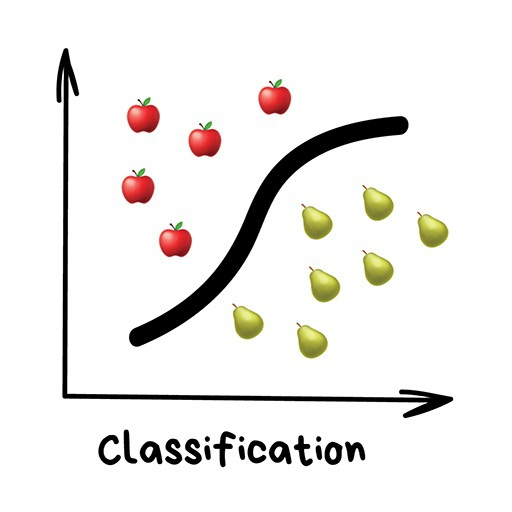
\includegraphics[width=0.2\textwidth]{figures/ml/7qx.jpg}};
%\node at (2,1) % reinforcement
%{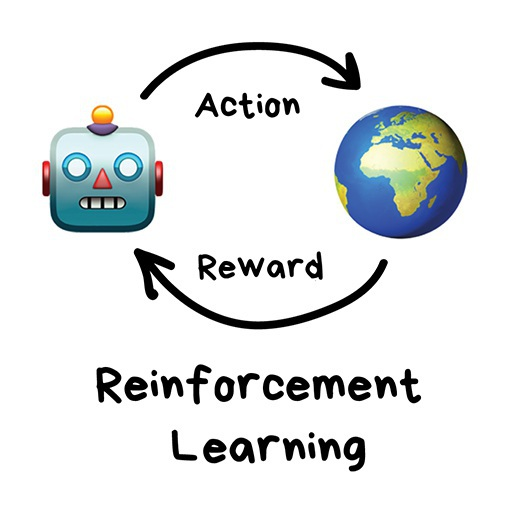
\includegraphics[width=0.2\textwidth]{figures/ml/7r2.jpg}};
%\node at (-2.2,1) % neural
%{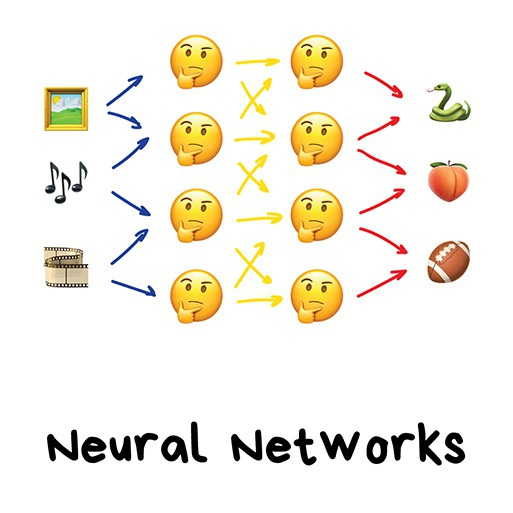
\includegraphics[width=0.2\textwidth]{figures/ml/7r4.jpg}};
%%\node at (-1.5,-1)
%%{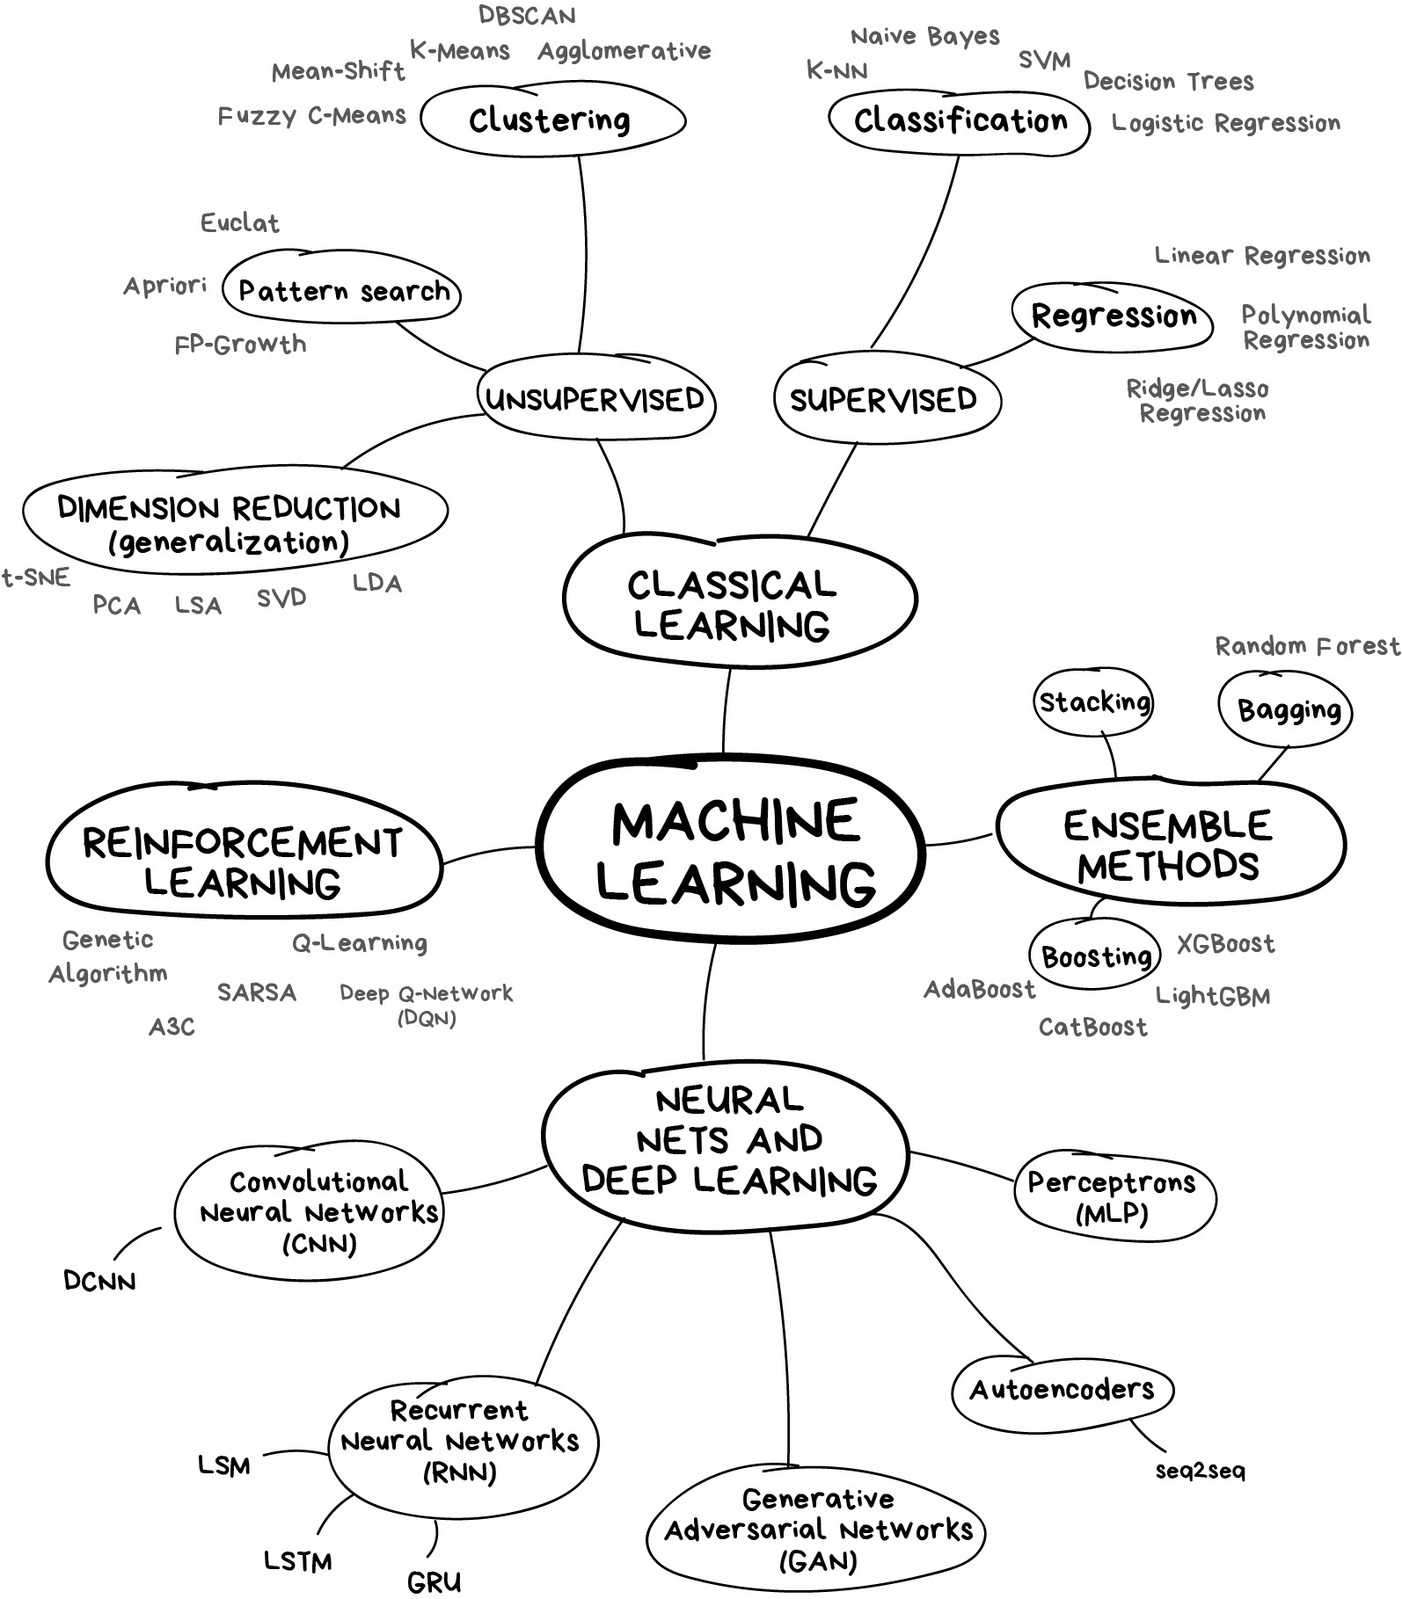
\includegraphics[width=0.15\textwidth]{figures/ml/7vx.jpg}};
%\node at (3,-1.25) % regression
%{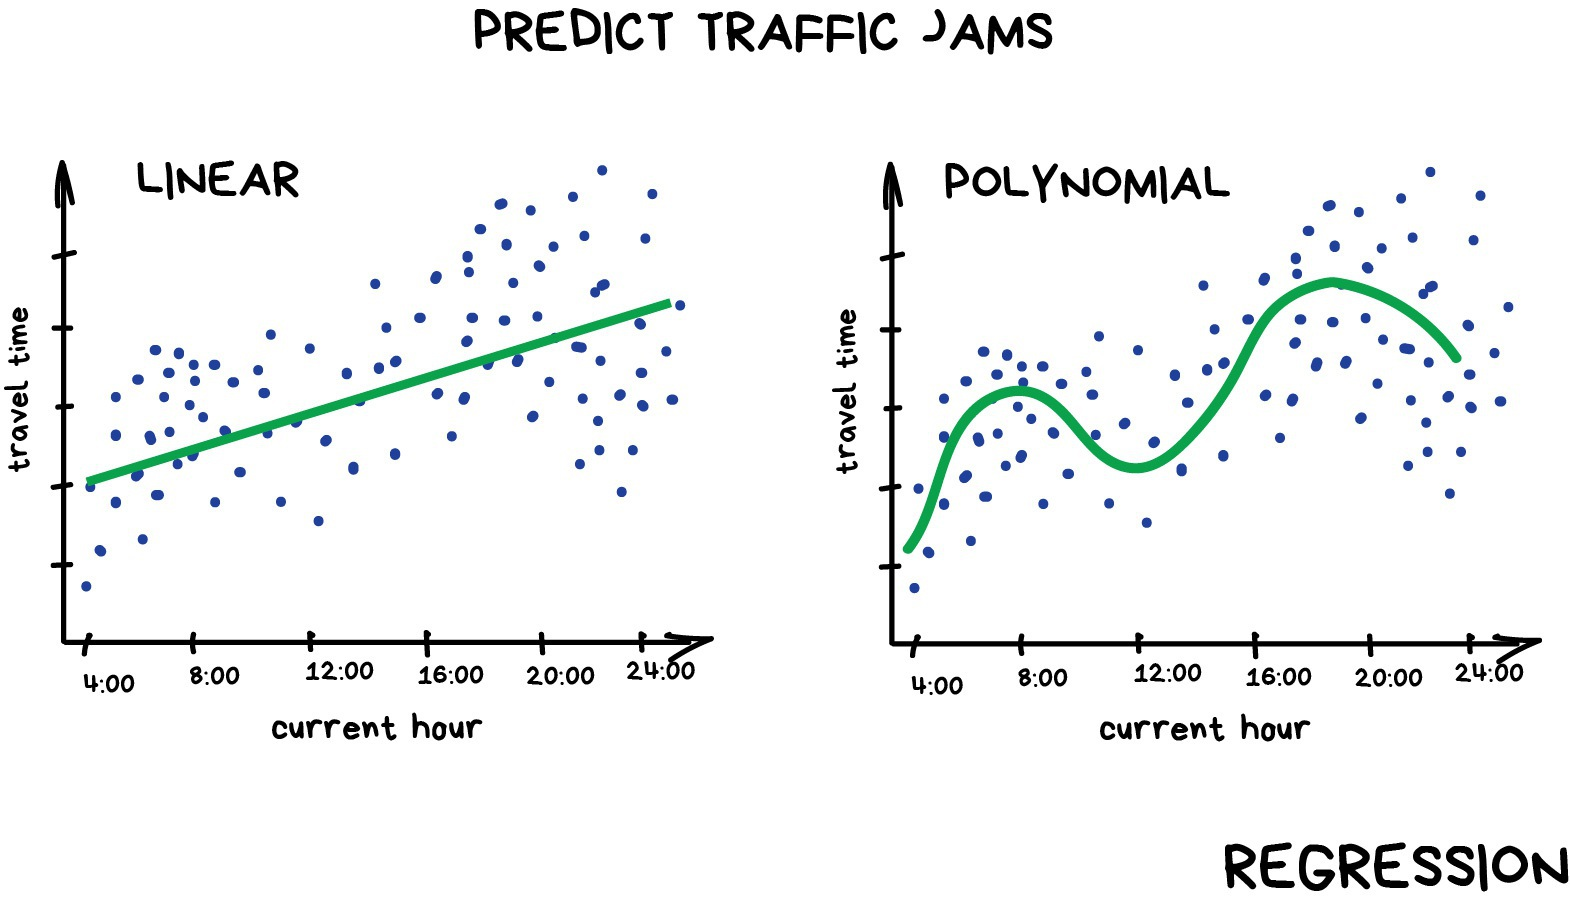
\includegraphics[width=0.35\textwidth]{figures/ml/7w5.jpg}};
%\node at (-3.25,-2.5) % multilayer
%{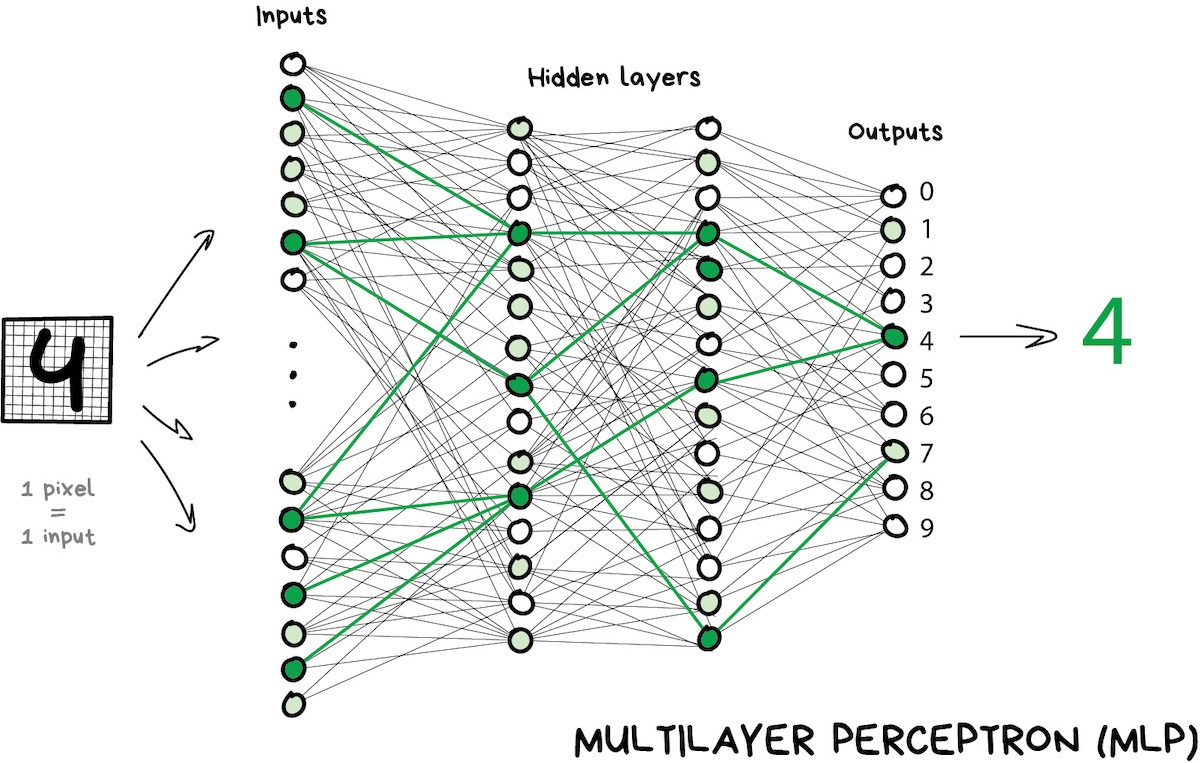
\includegraphics[width=0.4\textwidth]{figures/ml/7wg.jpg}};
%\node at (1.5,-3.5) % recurrent
%{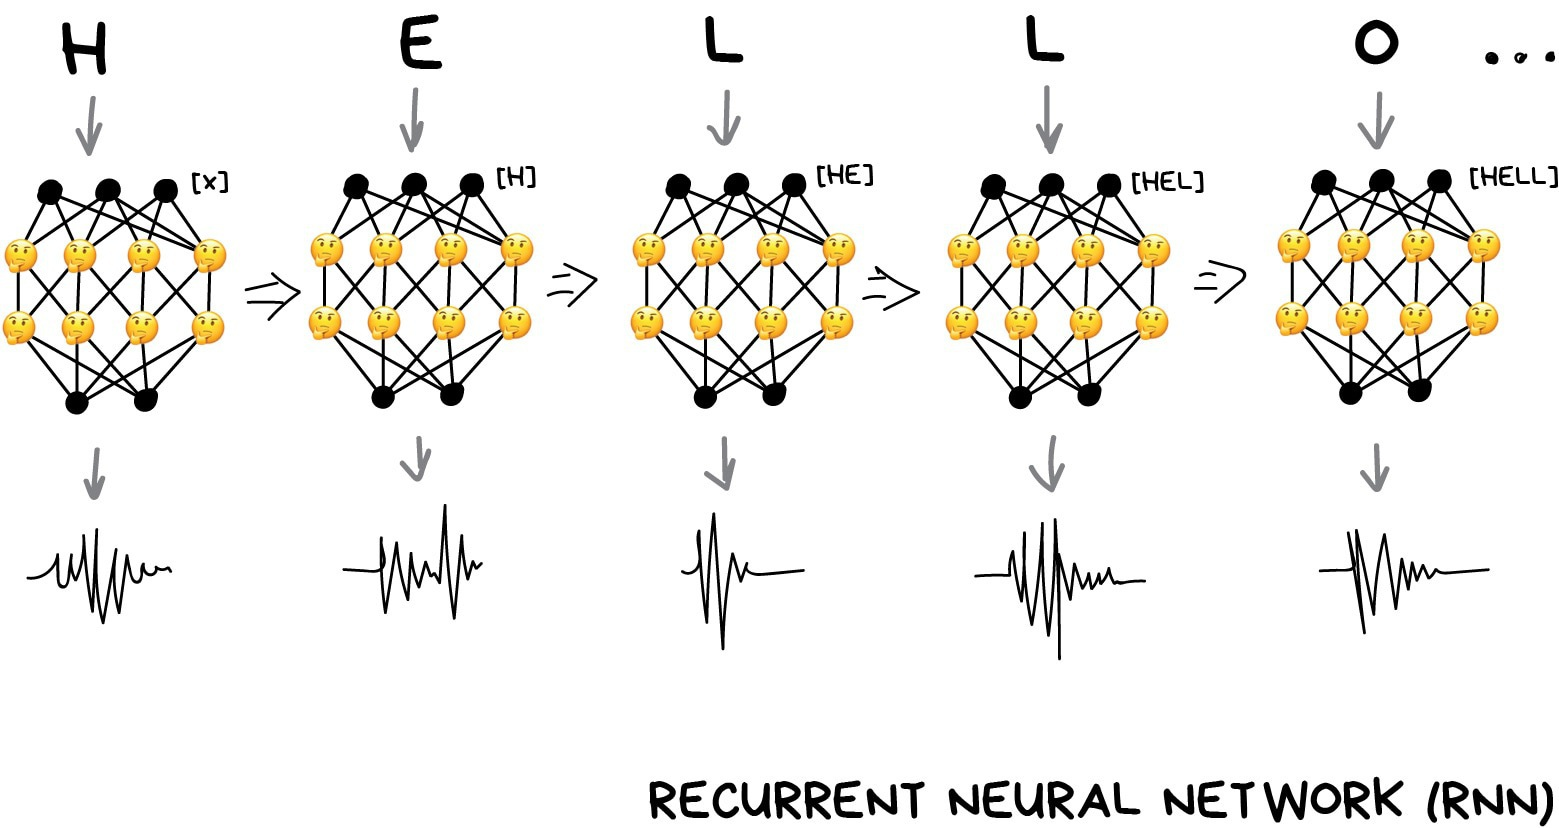
\includegraphics[width=0.4\textwidth]{figures/ml/7wk.jpg}};
%\node at (4.2,1.5) % clustering
%{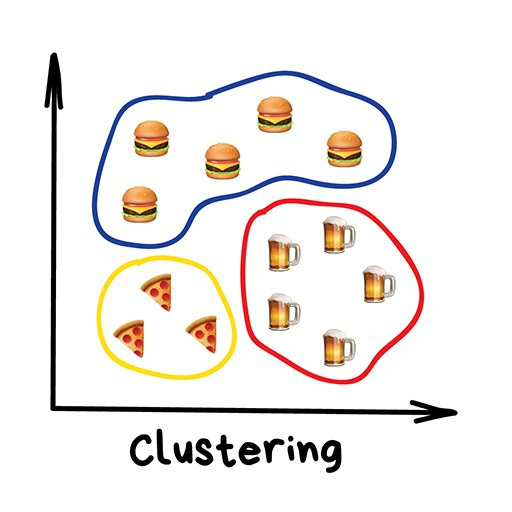
\includegraphics[width=0.2\textwidth]{figures/ml/7qz.jpg}};
%\node at (-4.5,0.25) % ensemble
%{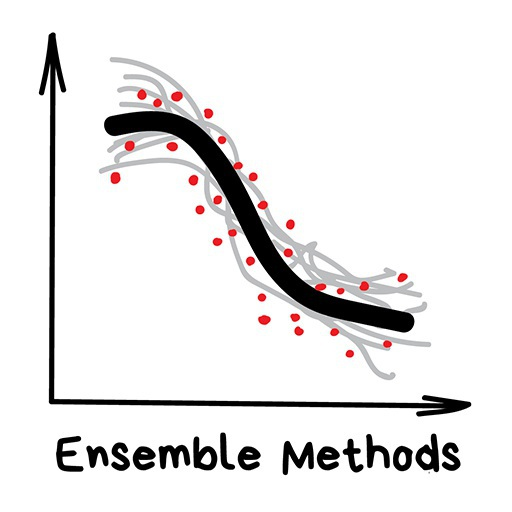
\includegraphics[width=0.2\textwidth]{figures/ml/7r3.jpg}};
%\node at (-4,3) %bayes
%{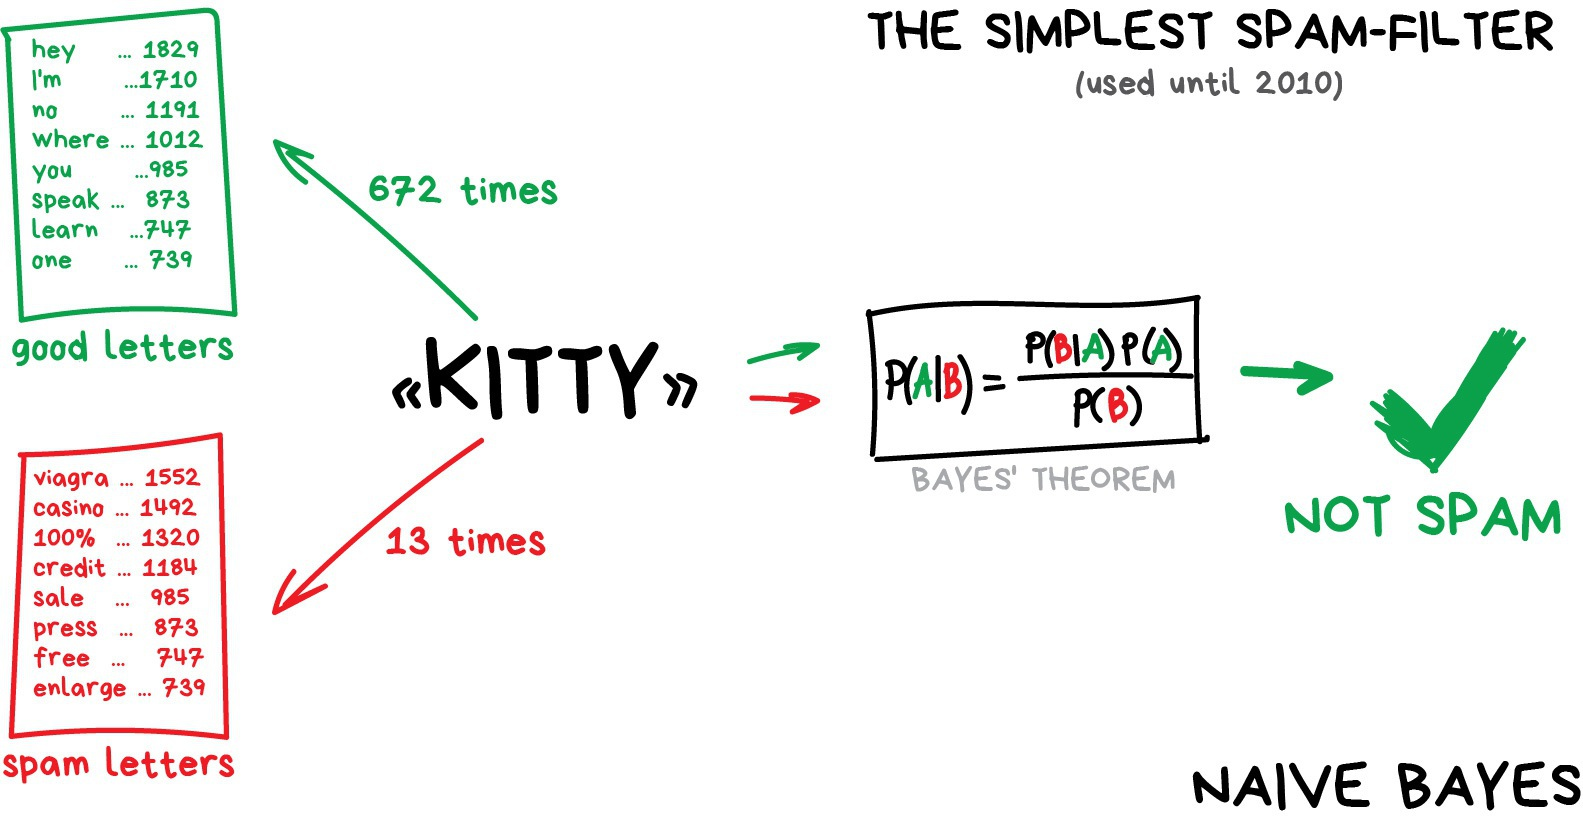
\includegraphics[width=0.3\textwidth]{figures/ml/7w2.jpg}};
%\node at (0,3.1) %stacking
%{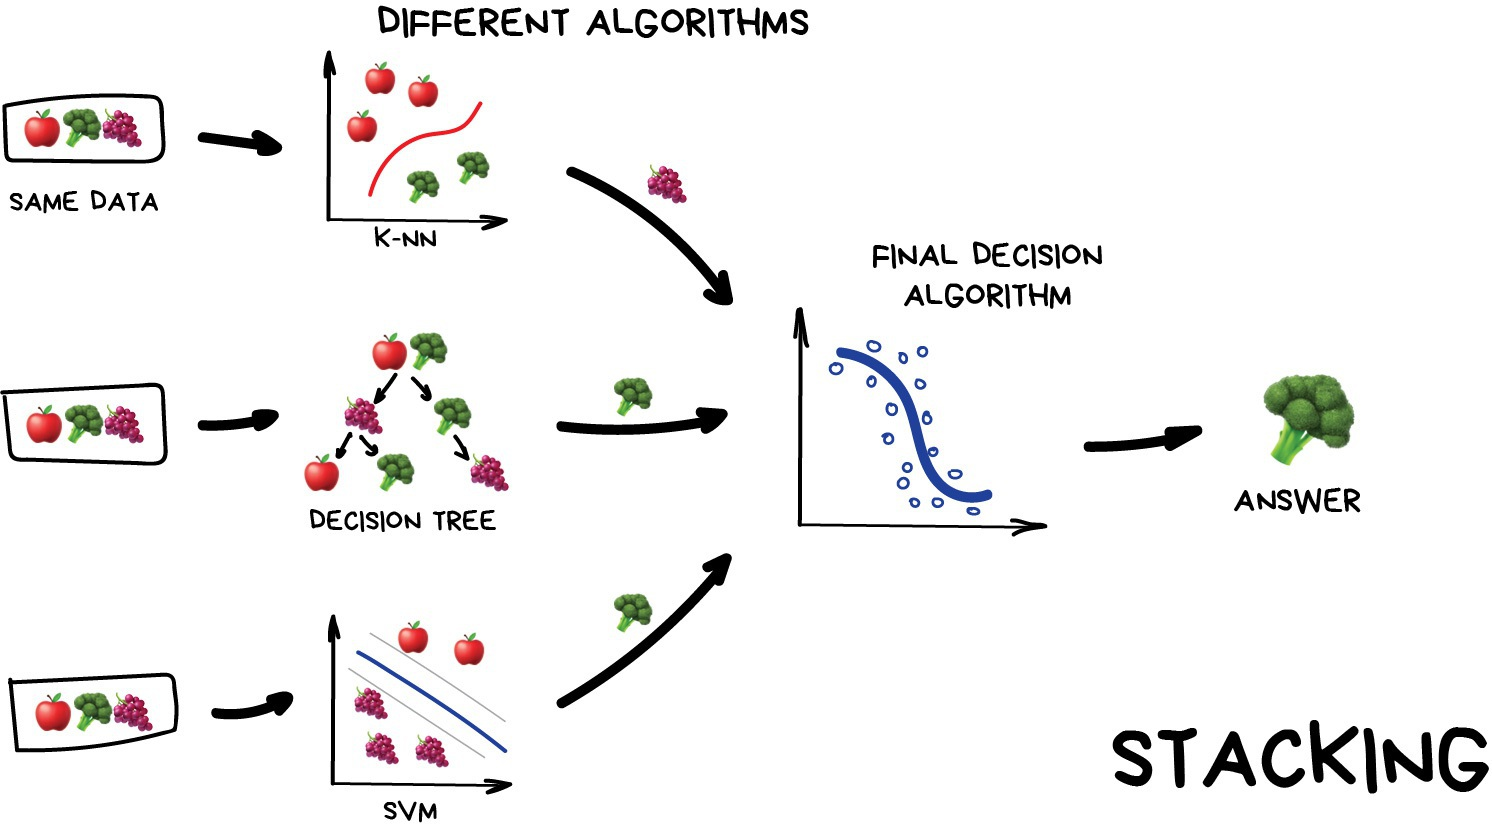
\includegraphics[width=0.3\textwidth]{figures/ml/7wb.jpg}};
%\node at (4,3.5) % convolution neural network
%{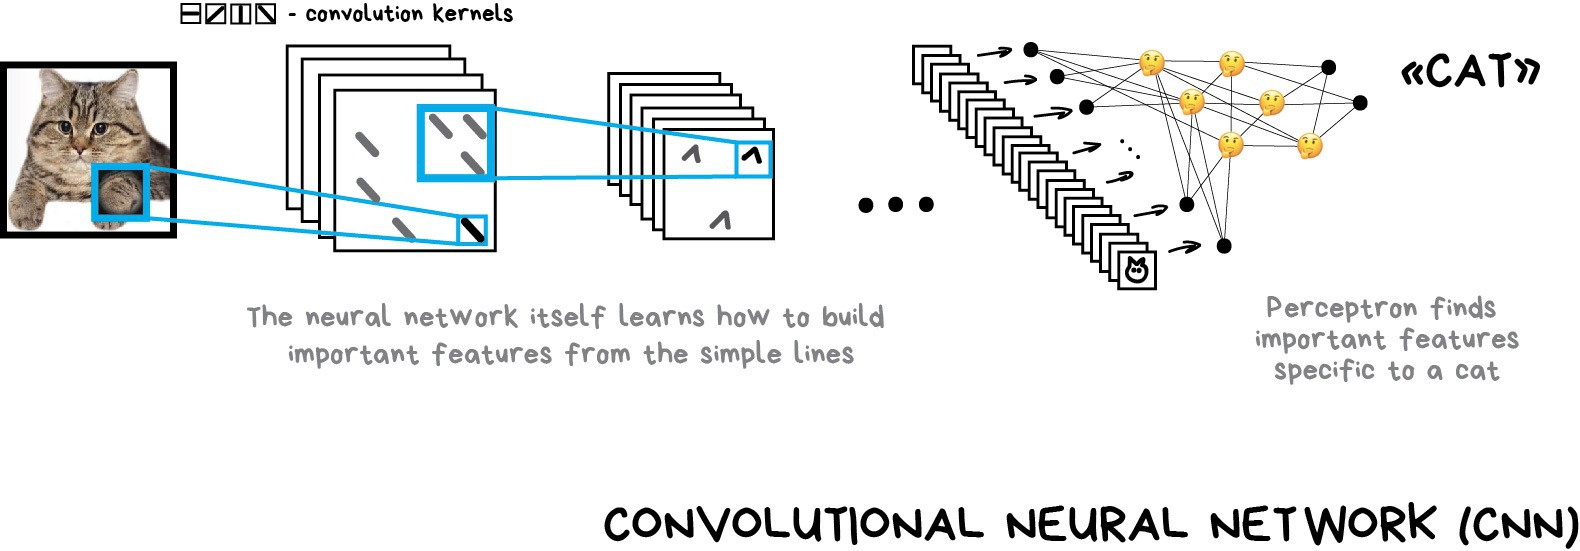
\includegraphics[width=0.4\textwidth]{figures/ml/7wj.jpg}};
%\end{tikzpicture}

%\end{frame}
%%%%%%%%%%%%%%%%%%%%%%%%%%%%%%%%%%%%%%%%%%%%%%%%%%%%%%%%%%%%%%%%%%%%%%%%
\section{DIM}
%%%%%%%%%%%%%%%%%%%%%%%%%%%%%%%%%%%%%%%%%%%%%%%%%%%%%%%%%%%%%%%%%%%%%%%%
\framecard[orange(colorwheel)]{{\color{white}
{\Huge \bf Problema 1:} 
\\ \vspace{0.5cm} 
{\LARGE \bf Potenciales efectivos \\\vspace{0.25cm} (DIM)}}}
%%%%%%%%%%%%%%%%%%%%%%%%%%%%%%%%%%%%%%%%%%%%%%%%%%%%%%%%%%%%%%%%%%%%%%%%
\framepic[1.]{figures/ionization.png}{}
%%%%%%%%%%%%%%%%%%%%%%%%%%%%%%%%%%%%%%%%%%%%%%%%%%%%%%%%%%%%%%%%%%%%%%%%
\begin{frame}
\frametitle{Método de Inversión Depurada (DIM)}

\begin{tikzpicture}[remember picture, overlay]
  \tikzset{shift={(current page.center)},xshift=0cm,yshift=2.4cm}
  \node<1-> (schro) 
  {\begin{minipage}{\textwidth}
\begin{center}
     $\left[ -\frac{1}{2} \frac{d^2}{d r^2} + \frac{l(l+1)}{2 r^2} 
      + {\color{red}V_{nl}(r)} \right] \, P_{nl}(r) = 
      E_{nl} \, P_{nl}(r)$
\end{center}
   \end{minipage}};
  \node<2-> (znl) at (schro) [xshift=0cm,yshift=-1.5cm]
  {\begin{minipage}{\textwidth}
     \begin{equation*}
      {\color{red}V_{nl}(r)} = \frac{1}{2}\frac{P_{nl}''(r)}{P_{nl}(r)}
          -\frac{l(l+1)}{2 r^2} +E_{nl}
     \end{equation*}
   \end{minipage}};
  \node<3-> (coulomb) at (znl) [xshift=-1.9cm,yshift=-3cm]
  {\begin{minipage}{0.55\textwidth}
      \begin{figure}
        \includegraphics[width=\textwidth]{figures/dim/effcharge.eps}
      \end{figure}
   \end{minipage}};
  \node<3-> (coulomb) at (znl) [xshift=3.1cm,yshift=-2.5cm]
  {\begin{minipage}{0.5\textwidth}
      \begin{equation*}
       V(r) = -\frac{{\color{red}Z(r)}}{r} 
      \end{equation*}
   \end{minipage}};
\end{tikzpicture}

\end{frame}
%%%%%%%%%%%%%%%%%%%%%%%%%%%%%%%%%%%%%%%%%%%%%%%%%%%%%%%%%%%%%%%%%%%%%%%%
\begin{frame}
\frametitle{Houston, we have a problem!}

\vspace{-0.25cm}
\begin{tikzpicture}[remember picture,overlay]
  \tikzset{shift={(current page.center)},xshift=0cm,yshift=0.1cm}
  \node (img1) 
  {\includegraphics[width=0.95\textwidth]{figures/dim/wavefun2sKr.eps}};
  \node<1-> (eq1) at (img1) [yshift=1.4cm,xshift=1.5cm]
  {$V(r) = \frac{1}{2} \frac{P''(r)}{P(r)} + E $}; 
  \node[draw,circle,minimum size=1cm,inner sep=0pt] (eq2) at (img1) [yshift=3.25cm,xshift=4.5cm] 
  {Kr}; 
  \node<2-> (img2) at (img1.west) [xshift=2cm,yshift=-2.5cm]
  {\includegraphics[width=0.4\textwidth]{figures/dim/problem1-2sKr.eps}};
  \node<3-> (img3) at (img1.east) [xshift=-1.75cm,yshift=-2.5cm]
  {\includegraphics[width=0.4\textwidth]{figures/dim/problem2-2sKr.eps}};
\end{tikzpicture}

\end{frame}
%%%%%%%%%%%%%%%%%%%%%%%%%%%%%%%%%%%%%%%%%%%%%%%%%%%%%%%%%%%%%%%%%%%%%%%%
\begin{frame}
\frametitle{Depuraci\'on}

\begin{tikzpicture}[remember picture,overlay]
  \tikzset{shift={(current page.center)},xshift=0cm,yshift=0.25cm}
  \node (img1) 
  {\includegraphics[width=0.7\textwidth]{figures/dim/depuration2sN-a.eps}};
  \node[draw,circle,minimum size=1cm,inner sep=0pt] (name) at (img1) [yshift=3.2cm,xshift=3.4cm] 
  {N};
  \node<3-> (eq1) at (img1) [yshift=-3.4cm,xshift=0cm]
  {\begin{minipage}{0.50\textwidth}
     \begin{equation*}
       \tikzmarkin[draw=orange,fill=orange!10]{depuration}(0.21,-0.75)(-0.1,0.65)
        Z(r) = 1+\sum_{j} \alpha_j e^{-\beta_j r} 
       \tikzmarkend{depuration}
     \end{equation*}
   \end{minipage}};
  \node<3-> (img2) 
  {\includegraphics[width=0.7\textwidth]{figures/dim/depuration2sN-b.eps}};
  \node<2-> (asym) at (img1) [yshift=0cm,xshift=-1.1cm]
  { {\small $\Bigg\{ \!\! \begin{array}{c}
  \!\!\!\!Z_N :\, r=0 \\ 
  \,1 \,\,\,:\, r\rightarrow \infty\\ \end{array} $ } };
  \node<4-> (eq1) at (img1) [yshift=-3.4cm,xshift=0cm]
  {\begin{minipage}{0.50\textwidth}
     \begin{equation*}
       \tikzmarkin[draw=orange,fill=orange!10]{depuration}(0.21,-0.75)(-0.1,0.65)
       Z(r) = 1+\sum_{j} {\color{orange}{\mathbf{\boldsymbol\alpha_j}}} 
          e^{-{\color{orange}{\mathbf{\boldsymbol\beta_j}}} r} 
       \tikzmarkend{depuration}
     \end{equation*}
   \end{minipage}};
\end{tikzpicture}

\end{frame}
%%%%%%%%%%%%%%%%%%%%%%%%%%%%%%%%%%%%%%%%%%%%%%%%%%%%%%%%%%%%%%%%%%%%%%%%
\begin{frame}
\frametitle{Procedimiento}

\begin{tikzpicture}[remember picture, overlay,
  expl1/.style={draw=red,fill=orange!7,rounded corners,text width=3cm,
  minimum width=0.5cm, minimum height=0.7cm, text centered},
  arrow/.style={red,ultra thick,->,>=latex}]
  \tikzset{shift={(current page.center)},xshift=0cm,yshift=2.5cm}
  \node[expl1,text width=2cm] (inv) {Inversión};
  \node[expl1,text width=5.4cm] (rem) at (inv) [xshift=0cm,yshift=-1.4cm]
  {Remoción de divergencias};
  \node[expl1,text width=2.75cm] (var) at (rem) [xshift=0cm,yshift=-1.8cm]
  {Variación de parámetros};
  \node[expl1,text width=3.1cm] (diag) at (var) [xshift=2.5cm,yshift=-2cm]
  {Diagonalización};
  \node[expl1,text width=3.4cm] (err) at (var) [xshift=-2.5cm,yshift=-2cm]
  {Cálculo de costo};
  \draw [arrow, bend right=0] 
  ([xshift=0cm,yshift=0cm]{inv}) to ([xshift=0cm,yshift=0cm]{rem.north});
  \draw [arrow, bend right=0] 
  ([xshift=0cm,yshift=0cm]{rem}) to ([xshift=0cm,yshift=0cm]{var.north});
  \draw [arrow, bend right=-30] 
  ([xshift=0cm,yshift=0cm]{var.east}) to ([xshift=0cm,yshift=0cm]{diag.north});
  \draw [arrow, bend right=-40] 
  ([xshift=0cm,yshift=0cm]{diag}) to ([xshift=0cm,yshift=0cm]{err.south});
  \draw [arrow, bend right=-30] 
  ([xshift=0cm,yshift=0cm]{err}) to ([xshift=0cm,yshift=0cm]{var.west});
  \draw [arrow, bend right=-30,dashed] 
  ([xshift=-0.75cm,yshift=0cm]{err.north}) to ([xshift=0cm,yshift=-0.25cm]{rem.west});
\end{tikzpicture}

\end{frame}
%%%%%%%%%%%%%%%%%%%%%%%%%%%%%%%%%%%%%%%%%%%%%%%%%%%%%%%%%%%%%%%%%%%%%%%%
\framecard[colorblue]{{\color{white}
{\Huge \bf Problema 2:} 
\\ \vspace{0.5cm} 
{\LARGE \bf Cálculos colisionales \\\vspace{0.25cm} 
(R--Matrix)}}}
%%%%%%%%%%%%%%%%%%%%%%%%%%%%%%%%%%%%%%%%%%%%%%%%%%%%%%%%%%%%%%%%%%%%%%%%
\section{R--Matrix}
%%%%%%%%%%%%%%%%%%%%%%%%%%%%%%%%%%%%%%%%%%%%%%%%%%%%%%%%%%%%%%%%%%%%%%%%
\begin{frame}
\frametitle{R--Matrix}

\begin{columns}
\begin{column}{0.65\textwidth}

\begin{tikzpicture}[thick]
\tikzset{shift={(current page.center)},xshift=-2cm,yshift=0cm}
\node at (0,-0.65) {\footnotesize
$\begin{array}{c}\mbox{\it Núcleo del} \\ \mbox{\it blanco}\end{array}$};
\node at (0,0.75) {\footnotesize Región Interna};
\node at (0,2.2) {\footnotesize Región Externa};
\node at (-2.6,2.75) {\footnotesize 
$\begin{array}{c}
\mbox{electrón}\\
\mbox{incidente}
\end{array}$};
\node at (2.7,1.25) {\footnotesize 
$\begin{array}{c}
\mbox{electrón}\\
\mbox{dispersado}
\end{array}$};
\draw circle (1.75cm);
\draw[fill=darkgray] circle (0.1cm);
\draw[arrows=->,thick](-2.75,2.25)--(-1.5,1.4);
\draw[arrows=->,thick](1.5,1.4)--(2.75,2.25);
\end{tikzpicture}

\end{column}
\begin{column}{0.45\textwidth}  %%<--- here
\begin{tikzpicture}[remember picture,overlay,
  arrow/.style={red,ultra thick,->,>=latex}]
  \tikzset{shift={(current page.center)},xshift=3.25cm,yshift=2.25cm}
  \node (target) {Estructura del blanco};
  \node (auto) at (target) [xshift=0cm,yshift=-0.65cm] {\fbox{\sc \small autostructure}};
%
  \node (inner) at (target) [xshift=0cm,yshift=-2.25cm] {Región Interna};
  \node (rmatrxi) at (inner) [xshift=0cm,yshift=-0.65cm] {\fbox{\sc \small rmatrxi}};
%
  \node (outer) at (inner) [xshift=0cm,yshift=-2.25cm] {Región Externa};
  \node (stgf) at (outer) [xshift=0cm,yshift=-0.65cm] {\fbox{\sc \small stgf}};
%
  \draw [arrow, bend right=0] (auto) to ([xshift=0cm,yshift=0cm]{inner.north});
  \draw [arrow, bend right=0] (rmatrxi) to ([xshift=0cm,yshift=0cm]{outer.north});
\end{tikzpicture}

\end{column}
\end{columns}


\end{frame}
%%%%%%%%%%%%%%%%%%%%%%%%%%%%%%%%%%%%%%%%%%%%%%%%%%%%%%%%%%%%%%%%%%%%%%%%
\begin{frame}
\frametitle{Descripción del blanco}

\begin{tikzpicture}[remember picture,overlay,
  expl1/.style={draw=red,rounded corners,text width=0.15cm,
  minimum width=0.2, minimum height=0.4cm, text centered},
  expl2/.style={draw=red,rounded corners,text width=0.35cm,
  minimum width=0.25, minimum height=0.6cm, text centered},
  arrow/.style={red,ultra thick,->,>=latex}]
  \tikzset{shift={(current page.center)},xshift=0cm,yshift=1.5cm}
  \node (eqCI) 
  {\begin{minipage}{0.50\textwidth}
     \begin{equation*}
       \Psi_i(\mathbf{r}) =
       \sum_j^{N} c_{ji} \, \Phi_j(\mathbf{r})
     \end{equation*}
   \end{minipage}};
  \node<2-> (eqCI) 
  {\begin{minipage}{0.50\textwidth}
     \begin{equation*}
       \Psi_i(\mathbf{r}) =
       \sum_j^{\color{red}{N}} c_{ji} \, \Phi_j(\mathbf{r})
     \end{equation*}
   \end{minipage}};
  \node<2->[expl1] (N) at (eqCI) [xshift=0.05cm,yshift=0.4cm] {\,};
  \node<2-> (nconf) at (eqCI) [xshift=3.cm,yshift=1cm] {\small\it Configuraciones};
  \draw<2-> [arrow, bend right=-30] 
  ([xshift=0.175cm,yshift=-0.05cm]{N.north}) to ([xshift=0.1cm,yshift=0.1cm]{nconf.west});
%% Pnl
  \node<3-> (pnl) at (eqCI) [xshift=-2.35cm,yshift=-2.25cm]
   {\begin{minipage}{0.50\textwidth}
     \begin{equation*}
       \left[ \frac{1}{2} \frac{d^2}{dr^2} - \frac{l(l+1)}{2r^2} 
     + V_{nl}^{\mbox{\scriptsize eff}}(\lambda_{nl},r)
 + E_{nl} \right] 
     P_{nl}(r)=0
     \end{equation*}
   \end{minipage}};
  \node<4-> (pnl) at (eqCI) [xshift=-2.35cm,yshift=-2.25cm]
   {\begin{minipage}{0.50\textwidth}
     \begin{equation*}
       \left[ \frac{1}{2} \frac{d^2}{dr^2} - \frac{l(l+1)}{2r^2} 
     + {\color{red}V_{nl}^{\mbox{\scriptsize eff}}(\lambda_{nl},r)}
 + E_{nl} \right] 
     P_{nl}(r)=0
     \end{equation*}
   \end{minipage}};
  \node<4-> (pot) at (pnl) [xshift=2.5cm,yshift=-2.2cm]
  {{\begin{varwidth}{\linewidth}
     \begin{itemize}
        \itemb Thomas–Fermi–Dirac–Amaldi 
        \itemb Slater-Type-Orbital de Burgess  
     \end{itemize}
    \end{varwidth}}}; 
  \node<5-> (pnl) at (eqCI) [xshift=-2.35cm,yshift=-2.25cm]
   {\begin{minipage}{0.50\textwidth}
     \begin{equation*}
       \left[ \frac{1}{2} \frac{d^2}{dr^2} - \frac{l(l+1)}{2r^2} 
     + {\color{red}V_{nl}^{\mbox{\scriptsize eff}}(\lambda_{nl},r)}
 + E_{nl} \right] 
     P_{nl}(r)=0
     \end{equation*}
   \end{minipage}};
  \node<5->[expl2] (lam) at (pnl) [xshift=2.75cm,yshift=-0.275cm] {\,};
  \node<5-> (param) at (pnl) [xshift=6cm,yshift=1cm] {\small\it Parámetro de escaleo};
  \draw<5-> [arrow, bend right=-40] 
  ([xshift=0.15cm,yshift=-0.01cm]{lam.north}) to ([xshift=0.1cm,yshift=0.cm]{param.west});
\end{tikzpicture}

\end{frame}
%%%%%%%%%%%%%%%%%%%%%%%%%%%%%%%%%%%%%%%%%%%%%%%%%%%%%%%%%%%%%%%%%%%%%%%%
\begin{frame}
\frametitle{Dependencia de CI ($N$)}

\begin{tikzpicture}[remember picture,overlay]
  \tikzset{shift={(current page.center)},xshift=1cm,yshift=-0.75cm}
  \node (be_config) 
  {\includegraphics[width=0.8\textwidth]{figures/rmatrix/example_conf.eps}};
  \node[draw,circle,minimum size=1cm,inner sep=0pt] (tag) at (be_config) 
  [xshift=3.75cm,yshift=4cm] {Be};
  \node (be_ecfgs) at (be_config) [xshift=-5.5cm,yshift=2.5cm]
  {\small$ 
    \begin{array}{l}
      1s^2 2s^2 \\
      1s^2 2snl \\
      1s^2 2p^2 \\
      1s^2 2pnl \\
    \end{array}\!\vast\} $};
\end{tikzpicture}

\end{frame}
%%%%%%%%%%%%%%%%%%%%%%%%%%%%%%%%%%%%%%%%%%%%%%%%%%%%%%%%%%%%%%%%%%%%%%%%
\begin{frame}
\frametitle{Dependencia de escaleo ($\lambda_{nl}$)}

\begin{tikzpicture}[remember picture,overlay]
  \tikzset{shift={(current page.center)},xshift=0cm,yshift=-0.5cm}
  \node<1> (be_levels) 
  {\includegraphics[width=0.8\textwidth]{figures/rmatrix/Be_levels.eps}};
  \node[draw,circle,minimum size=1cm,inner sep=0pt] (tag) at (be_levels) 
  [xshift=4.75cm,yshift=3.75cm] {Be};
  \node<2-> (be_var) at (be_levels) [xshift=0cm,yshift=-0.25cm]
  {\includegraphics[width=0.8\textwidth]{figures/rmatrix/example_var.eps}};
\end{tikzpicture}

\end{frame}
%%%%%%%%%%%%%%%%%%%%%%%%%%%%%%%%%%%%%%%%%%%%%%%%%%%%%%%%%%%%%%%%%%%%%%%%
\begin{frame}
\frametitle{Procedimiento}

\begin{tikzpicture}[remember picture, overlay,
  expl1/.style={draw=red,fill=orange!7,rounded corners,text width=3cm,
  minimum width=0.5cm, minimum height=0.7cm, text centered},
  arrow/.style={red,ultra thick,->,>=latex}]
  \tikzset{shift={(current page.center)},xshift=0.75cm,yshift=1.75cm}
  \node[expl1,text width=5.3cm] (defcfg) 
  {$\begin{array}{c}
   \mbox{Definición de} \\
   \mbox{configuración electrónica} \\
    \end{array}$};
  \node[expl1,text width=2.75cm] (var) at (defcfg) [xshift=0cm,yshift=-2.25cm]
  {Variación de parámetros};
  \node[expl1,text width=3.1cm] (diag) at (var) [xshift=2.5cm,yshift=-2cm]
  {Diagonalización};
  \node[expl1,text width=3.4cm] (err) at (var) [xshift=-2.5cm,yshift=-2cm]
  {Cálculo de costo};
  \draw [arrow, bend right=0] 
  ([xshift=0cm,yshift=0cm]{defcfg}) to ([xshift=0cm,yshift=0cm]{var.north});
  \draw [arrow, bend right=-30] 
  ([xshift=0cm,yshift=0cm]{var.east}) to ([xshift=0cm,yshift=0cm]{diag.north});
  \draw [arrow, bend right=-40] 
  ([xshift=0cm,yshift=0cm]{diag}) to ([xshift=0cm,yshift=0cm]{err.south});
  \draw [arrow, bend right=-30] 
  ([xshift=0cm,yshift=0cm]{err}) to ([xshift=0cm,yshift=0cm]{var.west});
  \draw [arrow, bend right=-30,dashed] 
  ([xshift=-0.75cm,yshift=0cm]{err.north}) to ([xshift=0cm,yshift=-0.25cm]{defcfg.west});
  \node[expl1,text width=2.25cm] (rmatrix) at (var) [xshift=-4.2cm,yshift=0.1cm]
  {R--Matrix};
\end{tikzpicture}

\end{frame}
%%%%%%%%%%%%%%%%%%%%%%%%%%%%%%%%%%%%%%%%%%%%%%%%%%%%%%%%%%%%%%%%%%%%%%%%
\begin{frame}
\frametitle{Síntesis del problema}

\begin{tikzpicture}[remember picture, overlay]
  \tikzset{shift={(current page.center)},xshift=0cm,yshift=1cm}
  \node (Jfunc) 
  {\begin{minipage}{\textwidth}
      Función de costo:
      \medskip
      \begin{equation*}
       J = \sum_j \left|\frac{\widetilde{E_j}(\boldsymbol{\xi}) 
      - E_j}{E_j} \right|
      \end{equation*}
   \end{minipage}};
  \node (exppar) at (Jfunc) [xshift=0cm,yshift=-3cm]
  {\begin{minipage}{\textwidth}
      \begin{itemize}
      \itemb DIM: $\boldsymbol{\xi}=\{\boldsymbol{\alpha},\boldsymbol{\beta} \}$
      \itemb R--Matrix: $\boldsymbol{\xi}=\{N,\boldsymbol{\lambda} \}$
      \end{itemize}
   \end{minipage}};
\end{tikzpicture}

\end{frame}
%%%%%%%%%%%%%%%%%%%%%%%%%%%%%%%%%%%%%%%%%%%%%%%%%%%%%%%%%%%%%%%%%%%%%%%%
\begin{frame}
\frametitle{Síntesis del problema}

\begin{tikzpicture}[remember picture, overlay]
  \tikzset{shift={(current page.center)},xshift=-2.5cm,yshift=1cm}
  \node (Jfunc) 
  {\begin{minipage}{0.5\textwidth}
      Función de costo:
      \medskip
      \begin{equation*}
       J = \sum_j \left|\frac{\widetilde{E_j}(\boldsymbol{\xi}) 
      - E_j}{E_j} \right|
      \end{equation*}
   \end{minipage}};
  \node (exppar) at (Jfunc) [xshift=0.75cm,yshift=-3cm]
  {\begin{minipage}{0.7\textwidth}
      \begin{itemize}
      \itemb DIM: $\boldsymbol{\xi}=\{\boldsymbol{\alpha},\boldsymbol{\beta} \}$
      \itemb R--Matrix: $\boldsymbol{\xi}=\{N,\boldsymbol{\lambda} \}$
      \end{itemize}
   \end{minipage}};
\end{tikzpicture}

\begin{tikzpicture}[remember picture, overlay,
  expl1/.style={draw=red,fill=orange!7,rounded corners,text width=3cm,
  minimum width=0.5cm, minimum height=0.1cm, text centered},
  arrow/.style={red,ultra thick,->,>=latex}]
  \tikzset{shift={(current page.center)},xshift=3.5cm,yshift=3cm}
  \node[expl1,text width=0.75cm,text height=0.1cm] (inv) 
  {\tiny Inversión};
  \node[expl1,text width=1.5cm,text height=0.1cm] (rem) at (inv) [xshift=0cm,yshift=-0.9cm]
  {\tiny Remoción};
  \node[expl1,text width=2.7cm,text height=0.1cm] (var) at (rem) [xshift=0cm,yshift=-0.9cm]
  {\tiny Variación de parámetros};
  \node[expl1,text width=1.7cm,text height=0.1cm] (diag) at (var) [xshift=1.5cm,yshift=-0.8cm]
  {\tiny Diagonalización};
  \node[expl1,text width=2cm,text height=0.1cm] (err) at (var) [xshift=-1.5cm,yshift=-0.8cm]
  {\tiny Cálculo de costo};
  \draw [arrow, bend right=0] 
  ([xshift=0cm,yshift=0cm]{inv}) to ([xshift=0cm,yshift=0cm]{rem.north});
  \draw [arrow, bend right=0] 
  ([xshift=0cm,yshift=0cm]{rem}) to ([xshift=0cm,yshift=0cm]{var.north});
  \draw [arrow, bend right=-30] 
  ([xshift=0cm,yshift=0cm]{var.east}) to ([xshift=0.5cm,yshift=0cm]{diag.north});
  \draw [arrow, bend right=-40] 
  ([xshift=0cm,yshift=0cm]{diag}) to ([xshift=0cm,yshift=0cm]{err.south});
  \draw [arrow, bend right=-30] 
  ([xshift=-0.5cm,yshift=0cm]{err.north}) to ([xshift=0cm,yshift=0cm]{var.west});
  \draw [arrow, bend right=-30,dashed] 
  ([xshift=-0.75cm,yshift=0cm]{err.north}) to ([xshift=0cm,yshift=-0.25cm]{rem.west});
\end{tikzpicture}

\begin{tikzpicture}[remember picture, overlay,
  expl1/.style={draw=red,fill=orange!7,rounded corners,text width=3cm,
  minimum width=0.5cm, minimum height=0.1cm, text centered},
  arrow/.style={red,ultra thick,->,>=latex}]
  \tikzset{shift={(current page.center)},xshift=3.8cm,yshift=-1.2cm}
  \node[expl1,text width=2.5cm,text height=0.1cm] (defcfg) 
  {\tiny Def. de config. elec.};
  \node[expl1,text width=2.5cm] (var) at (defcfg) [xshift=0cm,yshift=-1.cm]
  {\tiny Variación de parámetros};
  \node[expl1,text width=1.5cm] (diag) at (var) [xshift=1.3cm,yshift=-1cm]
  {\tiny Diagonalización};
  \node[expl1,text width=1.8cm] (err) at (var) [xshift=-1.3cm,yshift=-1cm]
  {\tiny Cálculo de costo};
  \draw [arrow, bend right=0] 
  ([xshift=0cm,yshift=0cm]{defcfg}) to ([xshift=0cm,yshift=0cm]{var.north});
  \draw [arrow, bend right=-20] 
  ([xshift=0cm,yshift=0cm]{var.east}) to ([xshift=0.4cm,yshift=0cm]{diag.north});
  \draw [arrow, bend right=-40] 
  ([xshift=0cm,yshift=0cm]{diag}) to ([xshift=0cm,yshift=0cm]{err.south});
  \draw [arrow, bend right=-30] 
  ([xshift=-0.4cm,yshift=0cm]{err.north}) to ([xshift=0cm,yshift=0cm]{var.west});
  \draw [arrow, bend right=-40,dashed] 
  ([xshift=-0.75cm,yshift=0cm]{err.north}) to ([xshift=0cm,yshift=-0.25cm]{defcfg.west});
  \node[expl1,text width=0.9cm] (rmatrix) at (var) [xshift=-2.5cm,yshift=0cm]
  {\tiny R--Matrix};
\end{tikzpicture}

\end{frame}
%%%%%%%%%%%%%%%%%%%%%%%%%%%%%%%%%%%%%%%%%%%%%%%%%%%%%%%%%%%%%%%%%%%%%%%%
\section{Procesos Gaussianos}
%%%%%%%%%%%%%%%%%%%%%%%%%%%%%%%%%%%%%%%%%%%%%%%%%%%%%%%%%%%%%%%%%%%%%%%%
\framecard[orange(colorwheel)]{{\color{white}
{\LARGE \bf Optimización Bayesiana} 
\\ \vspace{0.5cm} 
{\Large \bf con Procesos Gaussianos}}}
%%%%%%%%%%%%%%%%%%%%%%%%%%%%%%%%%%%%%%%%%%%%%%%%%%%%%%%%%%%%%%%%%%%%%%%%
\begin{frame}
\frametitle{Procesos Gaussianos}

\begin{tikzpicture}[remember picture, overlay]
  \tikzset{shift={(current page.center)},xshift=0cm,yshift=-0.5cm}
  \node<1> (func) {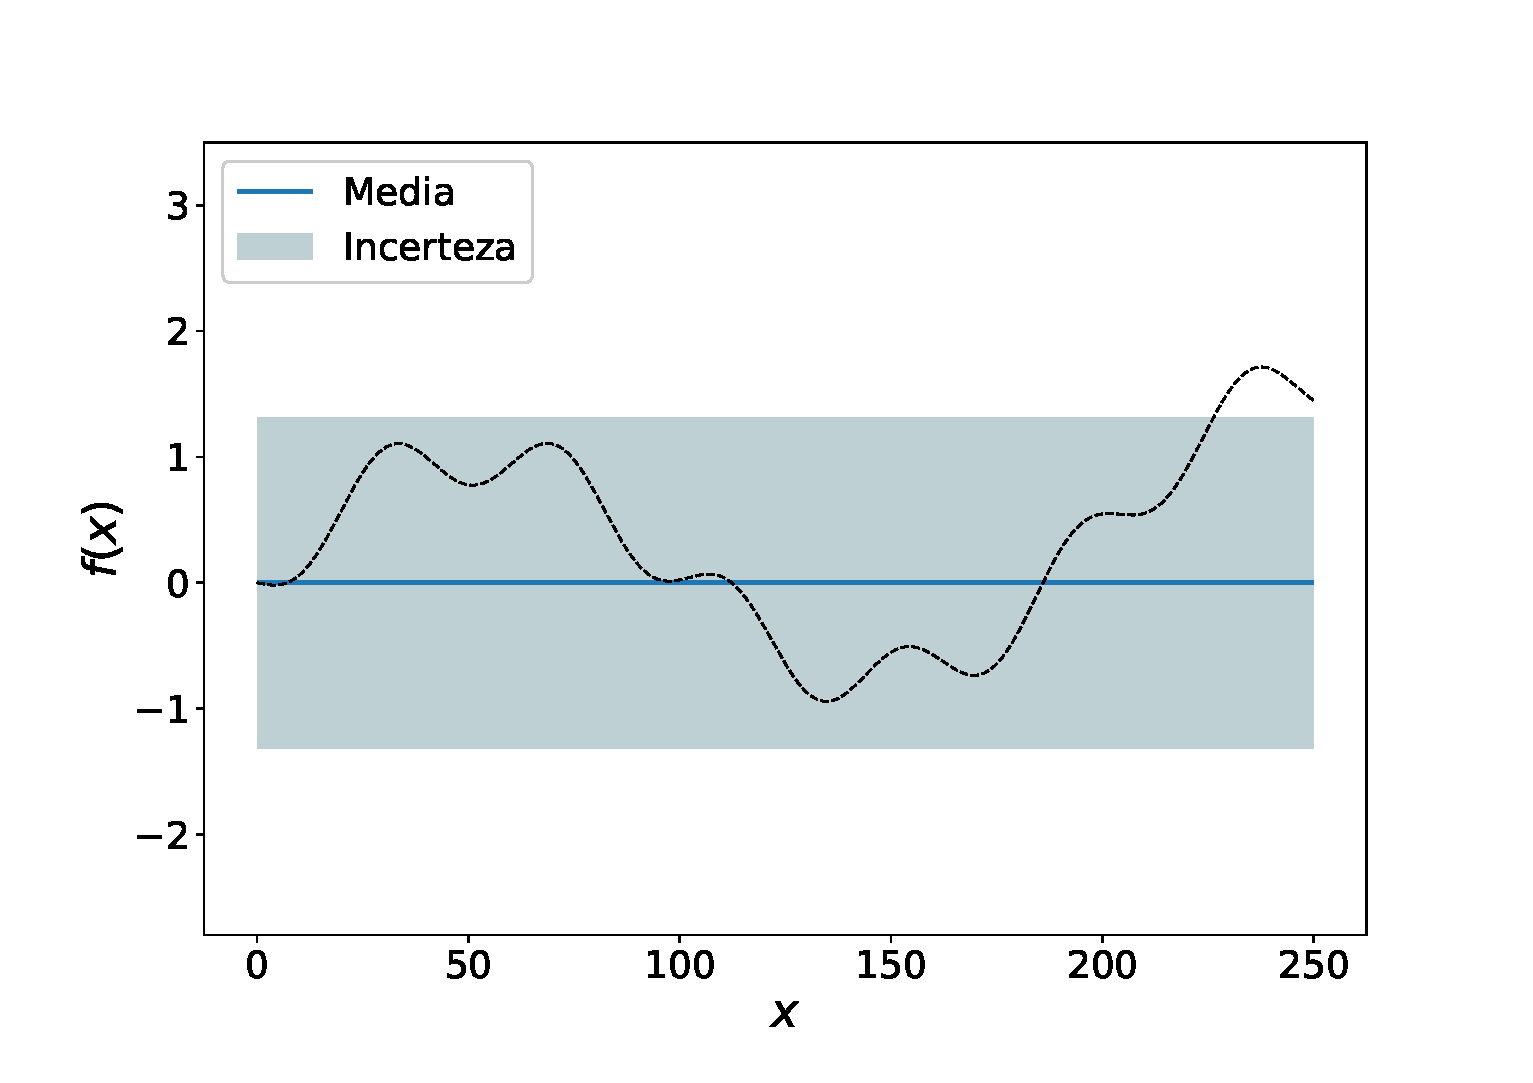
\includegraphics[width=\textwidth]{figures/gp/funcion.eps}};
  \node<2> (func) {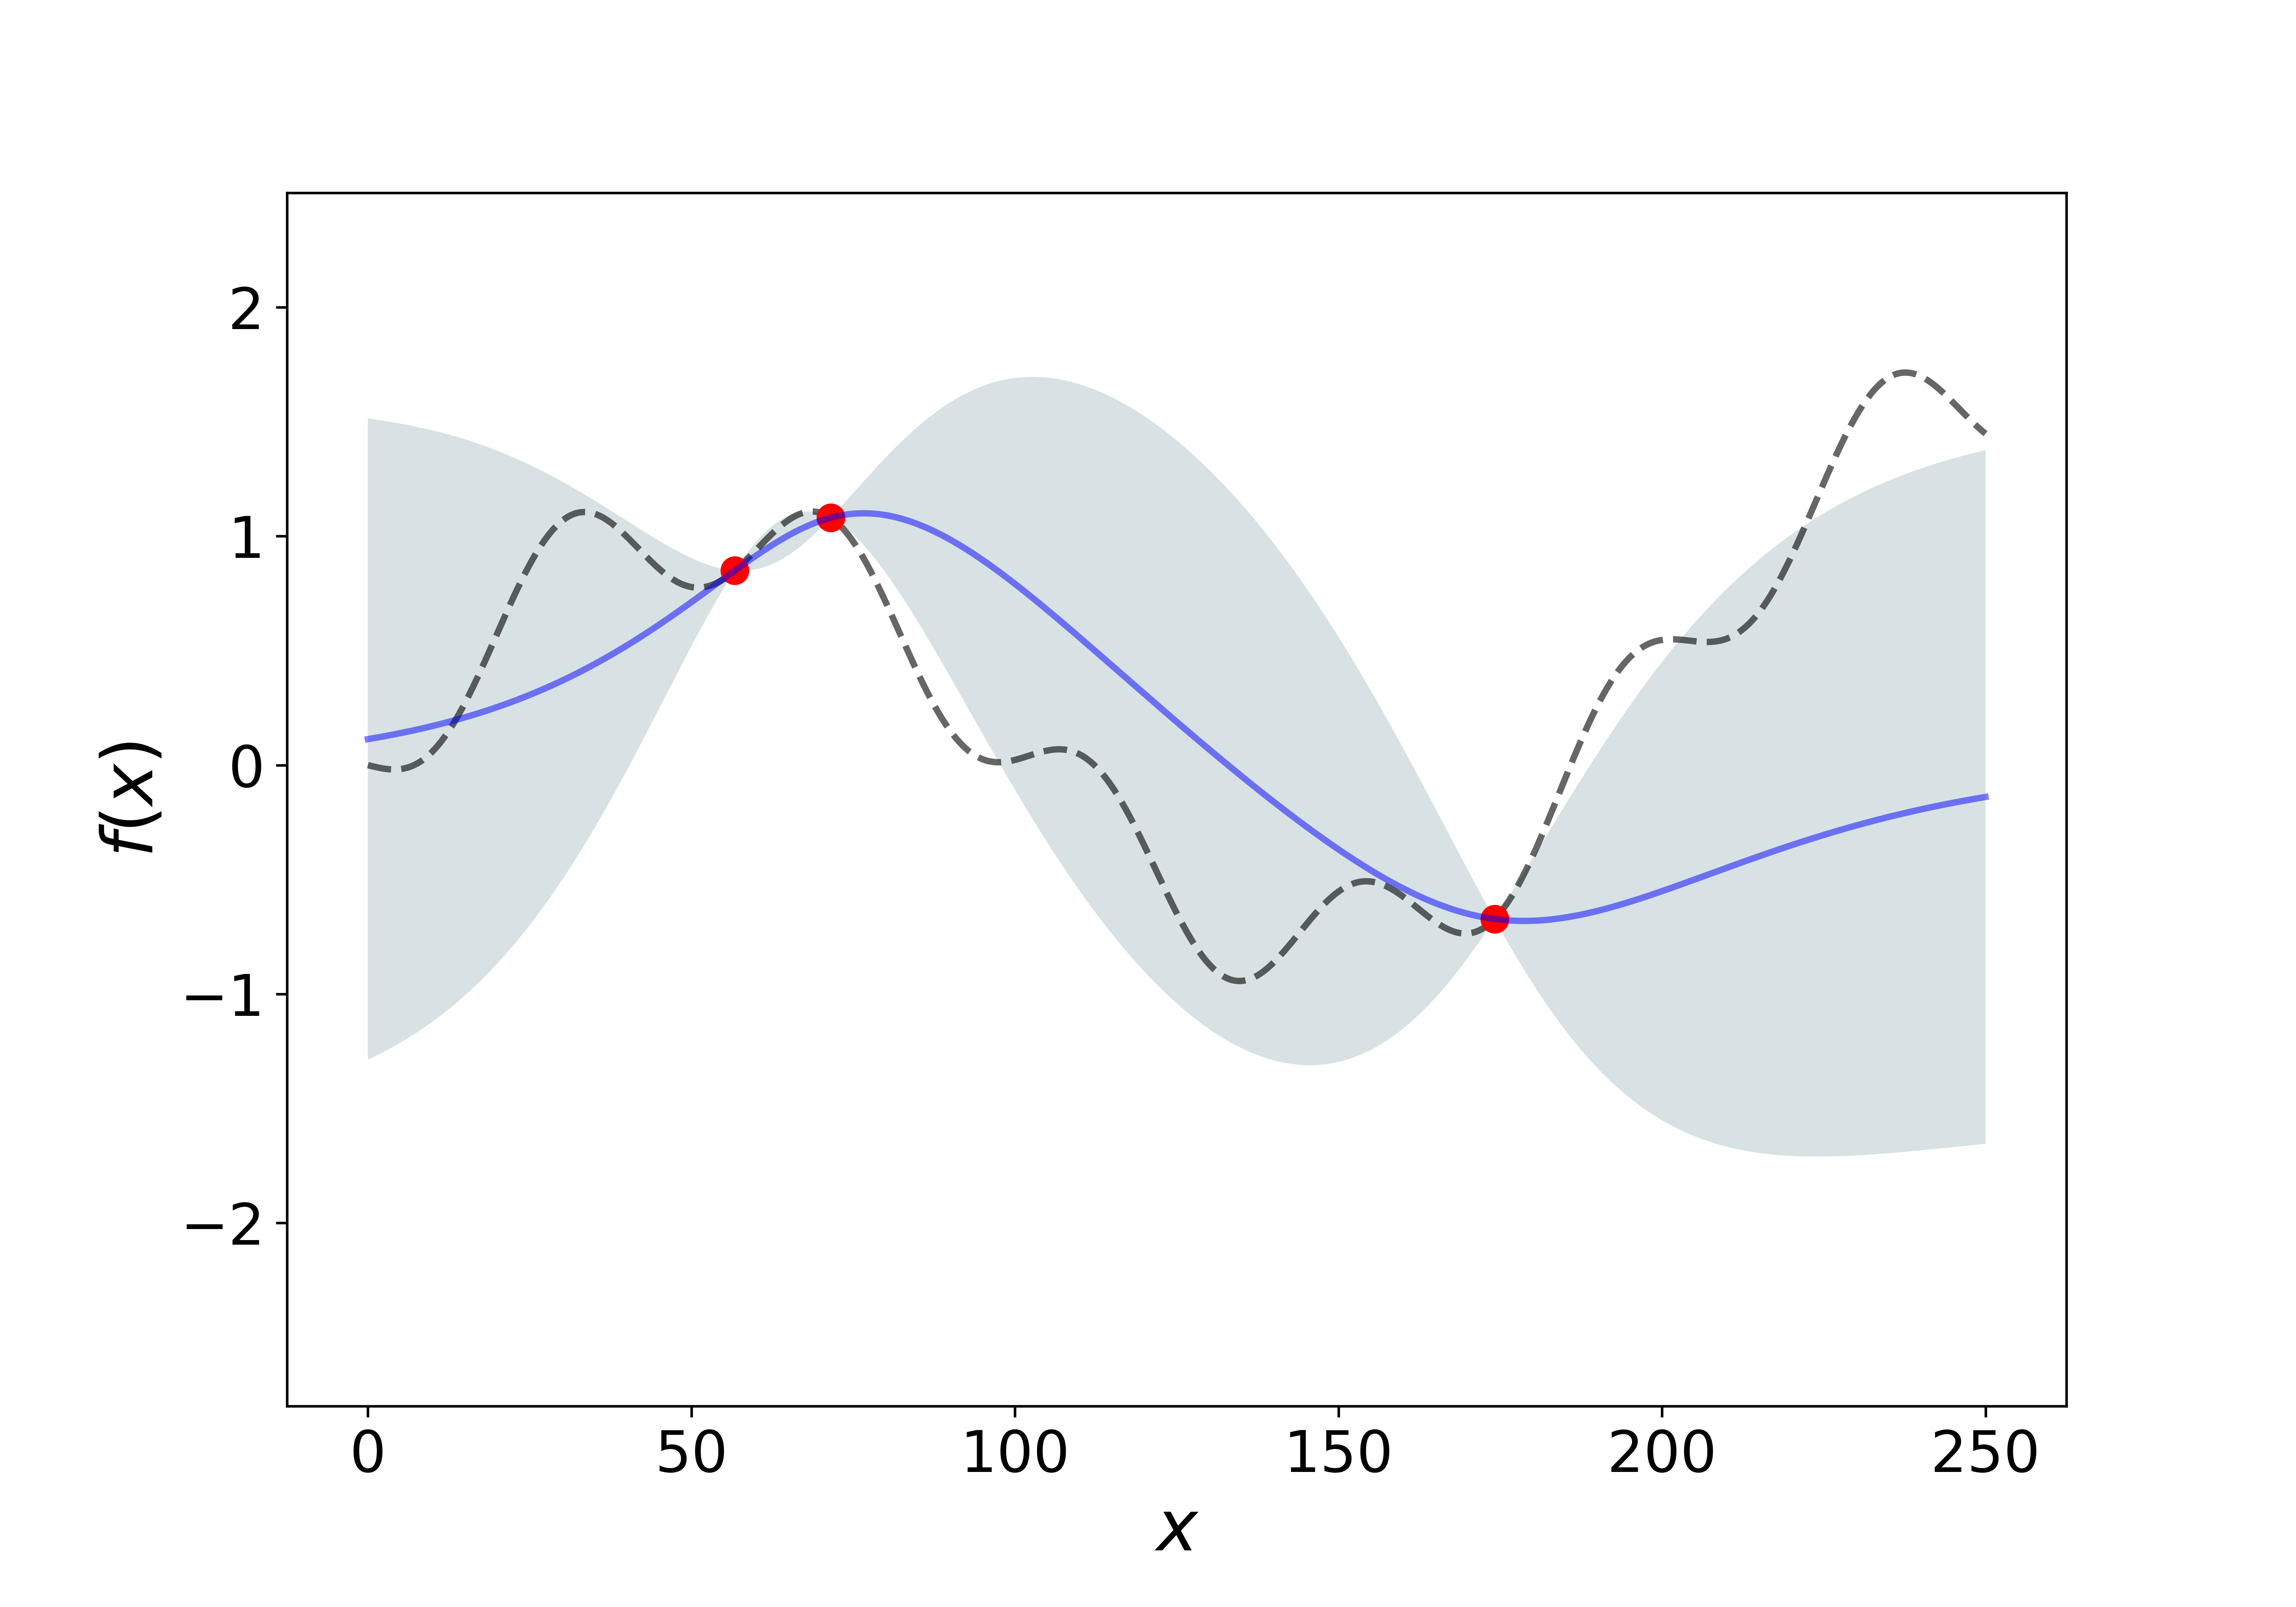
\includegraphics[width=\textwidth]{figures/gp/func_mean.eps}};
  \node<3> (func) {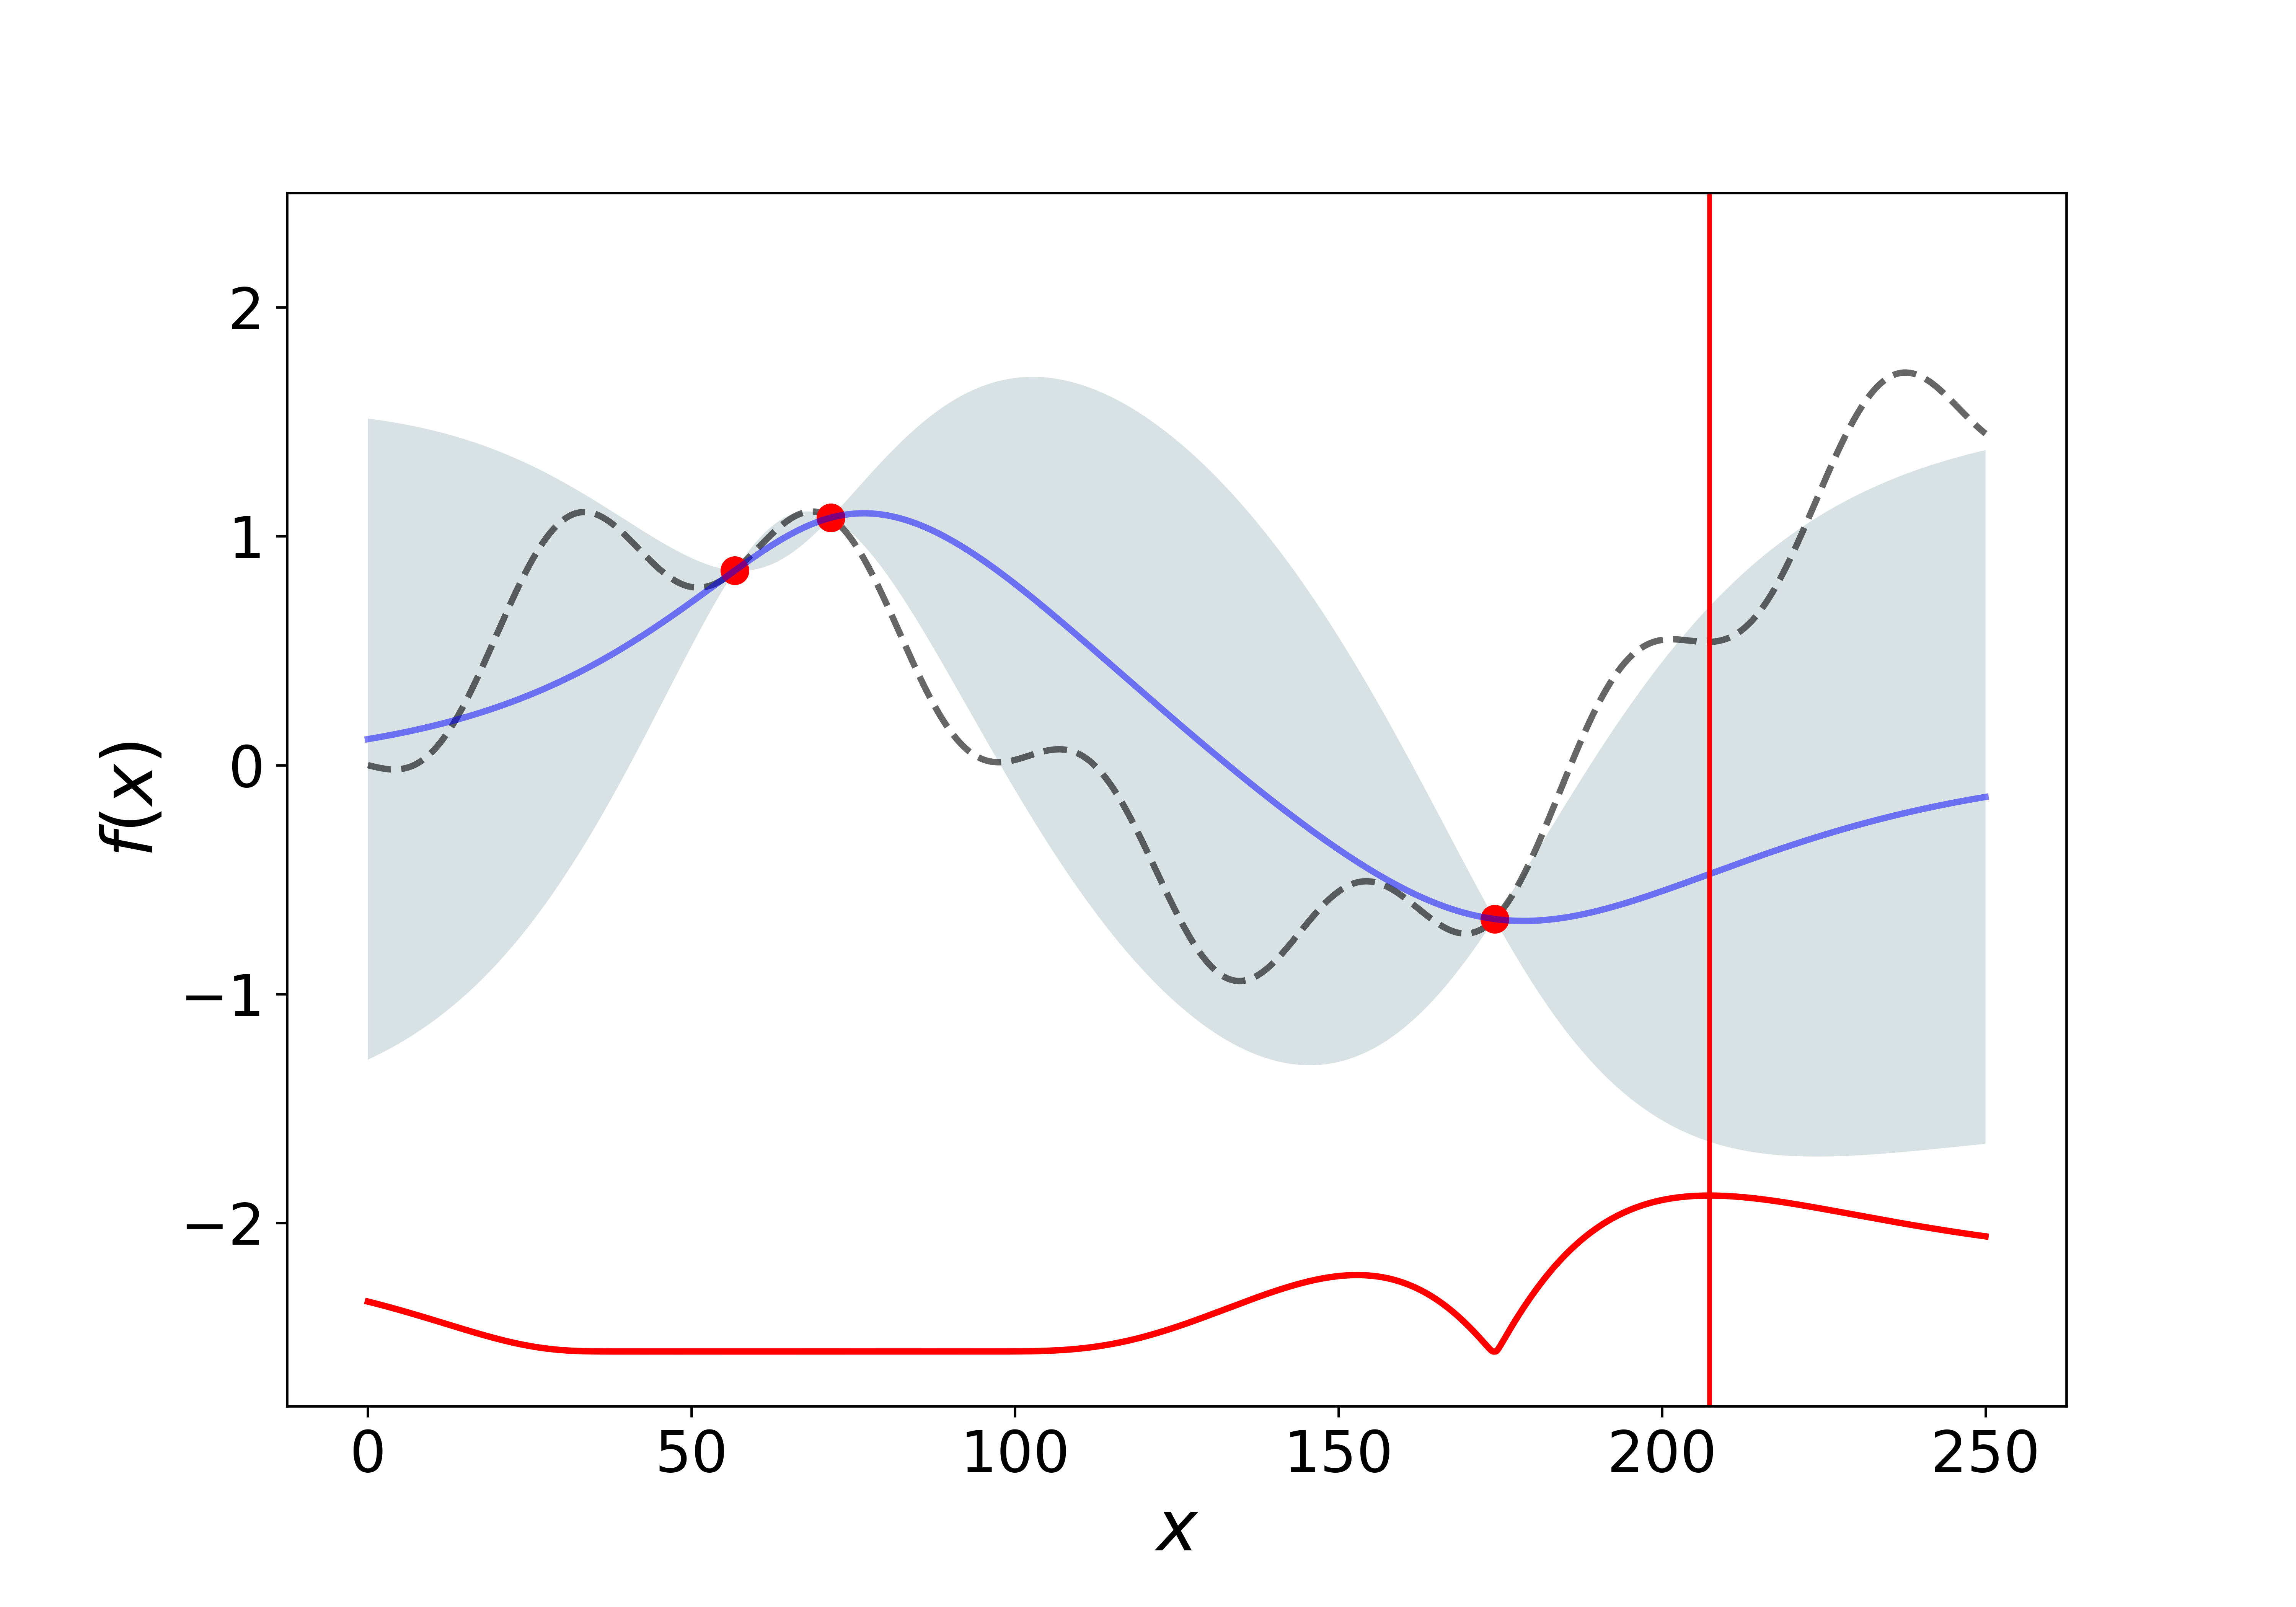
\includegraphics[width=\textwidth]{figures/gp/func_acq.eps}};
  \node<4> (max1) {\includegraphics[width=\textwidth]{figures/gp/eval1/example.eps}};
  \node<5> (max2) {\includegraphics[width=\textwidth]{figures/gp/eval2/example.eps}};
  \node<6> (max3) {\includegraphics[width=\textwidth]{figures/gp/eval3/example.eps}};
  \node<7> (max4) {\includegraphics[width=\textwidth]{figures/gp/eval4/example.eps}};
  \node<8> (max5) {\includegraphics[width=\textwidth]{figures/gp/eval5/example.eps}};
  \node<9> (max6) {\includegraphics[width=\textwidth]{figures/gp/eval6/example.eps}};
  \node<10> (max7) {\includegraphics[width=\textwidth]{figures/gp/eval7/example.eps}};
\end{tikzpicture}

\end{frame}
%%%%%%%%%%%%%%%%%%%%%%%%%%%%%%%%%%%%%%%%%%%%%%%%%%%%%%%%%%%%%%%%%%%%%%%%
%%%%%%%%%%%%%%%%%%%%%%%%%%%%%%%%%%%%%%%%%%%%%%%%%%%%%%%%%%%%%%%%%%%%%%%%
\section{Resultados}
%%%%%%%%%%%%%%%%%%%%%%%%%%%%%%%%%%%%%%%%%%%%%%%%%%%%%%%%%%%%%%%%%%%%%%%%
\framecard[colorgreen]{\color{white}
\LARGE \bf Resultados}
%%%%%%%%%%%%%%%%%%%%%%%%%%%%%%%%%%%%%%%%%%%%%%%%%%%%%%%%%%%%%%%%%%%%%%%%
\begin{frame}
\frametitle{DIM: Mg}

\begin{tikzpicture}[remember picture, overlay]
  \tikzset{shift={(current page.center)},xshift=-2.9cm,yshift=0.65cm}
  \node (1spot) 
  {\includegraphics[width=0.5\textwidth]{figures/dim/1s_pot.eps}};
  \node[draw,circle,minimum size=1cm,inner sep=0pt] (tag) at (1spot) [xshift=7.25cm,yshift=2.75cm]
  {$1s$};
  \node (1swfn) at (1spot) [xshift=5.6cm,yshift=0cm]
  {\includegraphics[width=0.5\textwidth]{figures/dim/1s_wfn.eps}};
  \node (1serr) at (1spot) [xshift=5.6cm,yshift=-3.18cm]
  {\includegraphics[width=0.5\textwidth]{figures/dim/error_1s.eps}};
  \node (error) at (1spot) [xshift=0cm,yshift=-3.25cm]
  {$\begin{array}{cc}
      E & {\Large\color{forestgreen(web)} \checkmark} \\
      \begin{array}{c}
        \langle r\rangle \\
        \langle 1/r \rangle
      \end{array} & 10^{-2} \%
    \end{array}$};
\end{tikzpicture}

\end{frame}
%%%%%%%%%%%%%%%%%%%%%%%%%%%%%%%%%%%%%%%%%%%%%%%%%%%%%%%%%%%%%%%%%%%%%%%%
\begin{frame}
\frametitle{DIM: Mg}

\begin{tikzpicture}[remember picture, overlay]
  \tikzset{shift={(current page.center)},xshift=-2.9cm,yshift=0.65cm}
  \node (1spot) 
  {\includegraphics[width=0.5\textwidth]{figures/dim/2s_pot.eps}};
  \node[draw,circle,minimum size=1cm,inner sep=0pt] (tag) at (1spot) [xshift=7.25cm,yshift=2.75cm]
  {$2s$};
  \node (1swfn) at (1spot) [xshift=5.58cm,yshift=0cm]
  {\includegraphics[width=0.505\textwidth]{figures/dim/2s_wfn.eps}};
  \node (1serr) at (1spot) [xshift=5.6cm,yshift=-3.11cm]
  {\includegraphics[width=0.5\textwidth]{figures/dim/error_2s.eps}};
  \node (error) at (1spot) [xshift=0cm,yshift=-3.25cm]
  {$\begin{array}{cc}
      E & {\Large\color{forestgreen(web)} \checkmark} \\
      \begin{array}{c}
        \langle r\rangle \\
        \langle 1/r \rangle
      \end{array} & 10^{-2} \%
    \end{array}$};
\end{tikzpicture}


\end{frame}
%%%%%%%%%%%%%%%%%%%%%%%%%%%%%%%%%%%%%%%%%%%%%%%%%%%%%%%%%%%%%%%%%%%%%%%%
\begin{frame}
\frametitle{DIM: Mg}

\begin{tikzpicture}[remember picture, overlay]
  \tikzset{shift={(current page.center)},xshift=-2.9cm,yshift=0.65cm}
  \node (1spot) 
  {\includegraphics[width=0.5\textwidth]{figures/dim/3s_pot.eps}};
  \node[draw,circle,minimum size=1cm,inner sep=0pt] (tag) at (1spot) [xshift=7.25cm,yshift=2.75cm]
  {$3s$};
  \node (1swfn) at (1spot) [xshift=5.58cm,yshift=0cm]
  {\includegraphics[width=0.505\textwidth]{figures/dim/3s_wfn.eps}};
  \node (1serr) at (1spot) [xshift=5.6cm,yshift=-3.11cm]
  {\includegraphics[width=0.5\textwidth]{figures/dim/error_3s.eps}};
  \node (error) at (1spot) [xshift=0cm,yshift=-3.25cm]
  {$\begin{array}{cc}
      E & {\Large\color{forestgreen(web)} \checkmark} \\
      \begin{array}{c}
        \langle r\rangle \\
        \langle 1/r \rangle
      \end{array} & 10^{-1} \%
    \end{array}$};
\end{tikzpicture}


\end{frame}
%%%%%%%%%%%%%%%%%%%%%%%%%%%%%%%%%%%%%%%%%%%%%%%%%%%%%%%%%%%%%%%%%%%%%%%%
\begin{frame}
\frametitle{R--Matrix: Be}

\vspace{-0.2cm}
\begin{figure}
\includegraphics[width=0.45\textwidth]{figures/rmatrix/sig001-002.eps} 
\hspace{0.3cm}
\includegraphics[width=0.45\textwidth]{figures/rmatrix/sig001-003.eps} \\
\vspace{0.1cm}
\includegraphics[width=0.45\textwidth]{figures/rmatrix/sig001-006.eps} 
\hspace{0.3cm}
\includegraphics[width=0.45\textwidth]{figures/rmatrix/sig001-007.eps}
\end{figure}

\end{frame}
%%%%%%%%%%%%%%%%%%%%%%%%%%%%%%%%%%%%%%%%%%%%%%%%%%%%%%%%%%%%%%%%%%%%%%%%
\begin{frame}
\frametitle{Conclusiones}

\begin{itemize}[<+-| alert@+>]
\itemb Estudiamos métodos y herramientas de aprendizaje automatizado
\vspace{0.2cm}
\itemb Implementamos estos métodos en problemas de física atómica
\vspace{0.2cm}
\begin{itemize}
  \itemb Método de Inversión Depurada
\vspace{0.2cm}
  \itemb Estructura del blanco en R--Matrix
\end{itemize}
\itemb El éxito en estos ejemplos sugiere que estos métodos se podrían 
utilizar en otros problemas del área
\vspace{0.2cm}
\end{itemize}

\end{frame}
%%%%%%%%%%%%%%%%%%%%%%%%%%%%%%%%%%%%%%%%%%%%%%%%%%%%%%%%%%%%%%%%%%%%%%%%
\framepic[1.]{figures/mlcover_modif.png}{
 \begin{textblock}{8}(6.,-1.5)
    {\color{orange0} 
\text{\huge \bf Gracias.} }
 \end{textblock}}
%%%%%%%%%%%%%%%%%%%%%%%%%%%%%%%%%%%%%%%%%%%%%%%%%%%%%%%%%%%%%%%%%%%%%%%%
\end{document}
